\chapter{Bluetooth Stack Implementation}
\label{chp:btstackimp}
\lhead{Chapter \ref{chp:btstackimp}. \emph{Bluetooth Stack Implementation}}

The development of the Bluetooth stack followed a bottom-up development methodology, designing and writing each software layer in sequence from the lowest layer first, to the highest and most abstracted layers last. This sequence ensured that each layer was functionally correct and could be verified before the higher layers were implemented. This suited the development of the Bluetooth stack---and, indeed, most software stacks---as each higher software layer is dependant solely on lower logical layers in the stack.

\section{Software Overview}

The software layers implemented in the completed Bluetooth stack are shown in Figure \ref{fig:completedbtstacklayers}.

\begin{figure}[tbph]
	\vspace{1em}
	\centering
		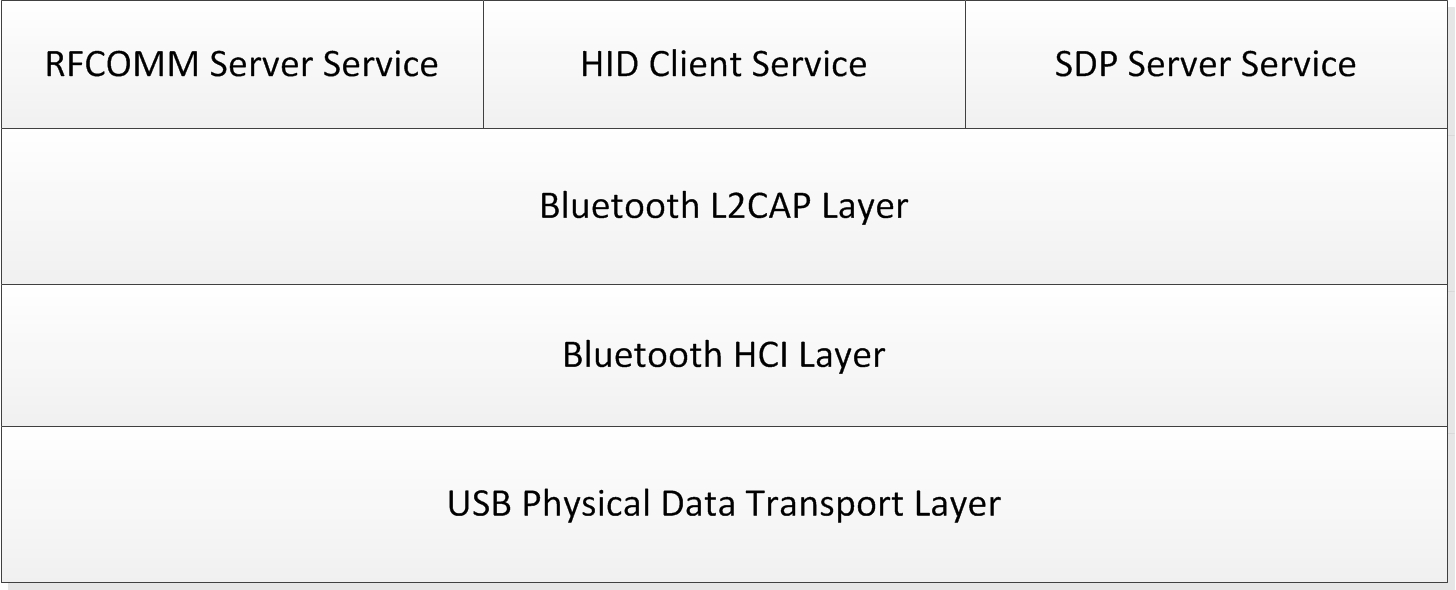
\includegraphics[width=100mm]{CompletedBluetoothStack.png}
	\rule{35em}{0.5pt}
	\caption[Diagram of the completed Bluetooth stack layers]{Diagram showing the completed layers of the Bluetooth stack.}
	\label{fig:completedbtstacklayers}
\end{figure}

Each software layer was implemented as a separate pair of source code module files, written in the C language and targeted towards the C99 language specification. Configuration for the stack is located in the file \texttt{BluetoothCommon.h}, which must be included in the user application to operate the stack.

By default, only the Bluetooth stack core (giving the HCI and L2CAP layers) is integrated; services must be linked into the stack manually via the provided event and callback routines (see later in this chapter) to provide service-level functionality on top of the base stack functionality. This includes the SDP server service; while generally a core requirement of most Bluetooth devices, it may be omitted in applications not exposing server role services to save space in the resulting application binary.

\section{Design Considerations}

A number of design restrictions were placed on the development of the Bluetooth stack; these ensured that the completed stack remained modular, extensible and suitable for integration in a wide range of embedded systems with various capabilities and, conversely, limitations. As an unfortunate but expected side effect, a number of these restrictions complicated the software development process significantly.

\FloatBarrier
\subsection{No Heap Memory Allocations}

The largest restriction placed on the stack design was the requirement of static and stack allocated memory allocation only --- no dynamic heap allocated memory was to be used via the usual \lstinline{malloc()} and \lstinline{free()} functions from the \texttt{libc} library. Most embedded environments contain three types of memory allocations:

\begin{enumerate}
	\item \textbf{Static Allocations}, including global variables and \lstinline{static} qualified variables.
	\item \textbf{Stack Allocations}, automatically populated to store local automatic variables, function parameters, return addresses, etc.
	\item \textbf{Heap Allocations}, persistent dynamic allocations manually managed by the user application.
\end{enumerate}

However, for significantly memory constrained systems, heap allocations are generally avoided due to the possibility of memory fragmentation; large numbers of differently-sized allocations and deallocations may cause fragmented holes to appear within the heap environment, causing allocation exhaustion to occur even if sufficient (raw) memory is available for an allocation request. In addition, dynamic memory complicates the formal analysis of a program, making memory requirements harder to judge, and thus harder to determine whether a given set of firmware will operate correctly within a specified environment without further in-depth analysis. In large embedded environments (ones with virtual memory management, and/or a large heap space) these problems are less of an issue and dynamic memory may be preferable for its simplicity.

The design of embedded stacks based on a no-heap-allocation strategy is a complex one, requiring certain trade-offs to be made. In the case of the Bluetooth stack presented here, a major side-effect of this decision was the need to fix the maximum number of simultaneous HCI device connections, L2CAP channel connections, and other queue- and list-like data structures within each instance of the stack. A major downside to this approach is the increased complexity of packet buffering and re-assembly, as fixed-size buffers must be used.

\FloatBarrier
\subsection{Endianness Correction}

A second complication based on the physical constraints from the execution environment is the native endianness of the processor hardware, i.e., the order in which multiple-byte data values are stored and interpreted inside the processor registers. Depending on the execution architecture, data values may be represented in Big Endian (most significant byte at the lowest address) or Little Endian (least significant byte at the lowest address) format within the CPU. Data transmitted and received at the local device to remote device boundary must undergo a encoding conversion if the endianness of the source and sink do not match.

In the case of the Bluetooth specification \cite{bt2p1specs}, this was further complicated by the various layers; some layers used Little Endian encoding for exchanged data, while others selected a Big Endian format. To perform the correct encoding/decoding on each platform, a set of conversion macros were implemented at points where multi-byte values were exchanged. This ensured that regardless of the native endian format of the architecture the stack is compiled to, multi-byte values will be interpreted correctly.

\FloatBarrier
\subsection{Physical Transport Independence}

As the Bluetooth 2.1 specification outlines a several possible physical transports \cite{bt2p1specs_transports} of HCI packets between the Bluetooth transceiver silicon and the application microcontroller, it was important that the physical transport layer be made independent from the rest of the stack. By making no assumptions about the form of transport protocol used to transfer packets to and from the attached Bluetooth silicon, the user application is free to implement their own transport mechanism without having to modify the internals of the stack. One instance of the stack may run across a USB connection to an attached Bluetooth module, while another may simultaneously connect to the microcontroller over a UART link.

\FloatBarrier
\subsection{Bluetooth Specification Compatibility}

For a software stack to be suitable for general use, it must be designed around, and undergo a series of tests to ensure compatibility with, a particular version of the protocol specification. Without a fixed version of a specification, correctness of the finished stack and compatibility with other implementations of the same technology cannot be assured.

As a \textit{compliant} stack would require extensive development and expensive certification procedures, the stack was instead aimed to be \textit{compatible} with version 2.1 of the Bluetooth specification. This subtle difference in the terminology indicates a large difference in the restrictions around the exact implementation. While a \textit{compliant} stack must be verified against the entire specification and rigorously tested to ensure exact conformance \cite{bt2p1specs_conformance}, a \textit{compatible} must only work with (most) other devices implementing their own compliant or compatible stacks of the same protocol version.

In the future the stack could be made conformant if desired, however for the purposes of the project only protocol compatibility was tested.

\FloatBarrier
\subsection{Multiple Stack Instances}

For maximum utility, the stack was designed to allow for multiple simultaneous stack instances. This was implemented to allow for unusual Bluetooth usage scenarios where more than one transceiver is desirable in a single system, either for security, wireless signal coverage or bandwidth reasons. Each physical transceiver is allocated a logical stack instance, capable of sustaining one or more simultaneous connections, and one or more logical channels between devices. This flexibility ensures that the majority of usage scenarios are covered by the stack's implementation.

Code-wise, the multiple stack functionality is implemented as a common first parameter to all functions within the stack, \lstinline{BT_StackConfig_t* const StackState}. This parameter is used to pass around a reference to the stack instance being operated upon, and is somewhat analogous to the \lstinline{this} property in C++ classes, if the entire stack was wrapped in a single class. As the stack was written in the C language which lacks Object Orientated language capabilities, this form of basic polymorphism was implemented manually. For each physical transceiver, the user application is expected to declare a new instance of the \lstinline{BT_StackConfig_t} structure within their code, and pass this to the main Bluetooth stack management routines (see Listing \ref{lst:stackconfig}).

\lstinputlisting[float=tbph,caption={Configuration example of a Bluetooth stack instance.},label={lst:stackconfig}]{./Figures/StackConfig.c}

\FloatBarrier
\subsection{Multiple Simultaneous Connections and Channels}

The HCI connections and L2CAP channels for each stack instance are implemented as an pair of object pools within the \lstinline{BT_StackConfig_t} structure; L2CAP channel objects within the pool are shared amongst all established HCI connections --- for example, one HCI connection may use all the available L2CAP channels, or two connections may share the pool equally. This design decision allows the full pool of L2CAP channel objects to be used by the stack regardless of the HCI connection requesting them. Figure \ref{fig:stackobjectpools} illustrates a single stack instance with a typical usage scenario, with two of the stack's HCI objects containing established connections, each with several L2CAP channel objects associated with the connection from the channel object pool.

\begin{figure}[tbph]
	\vspace{1em}
	\centering
		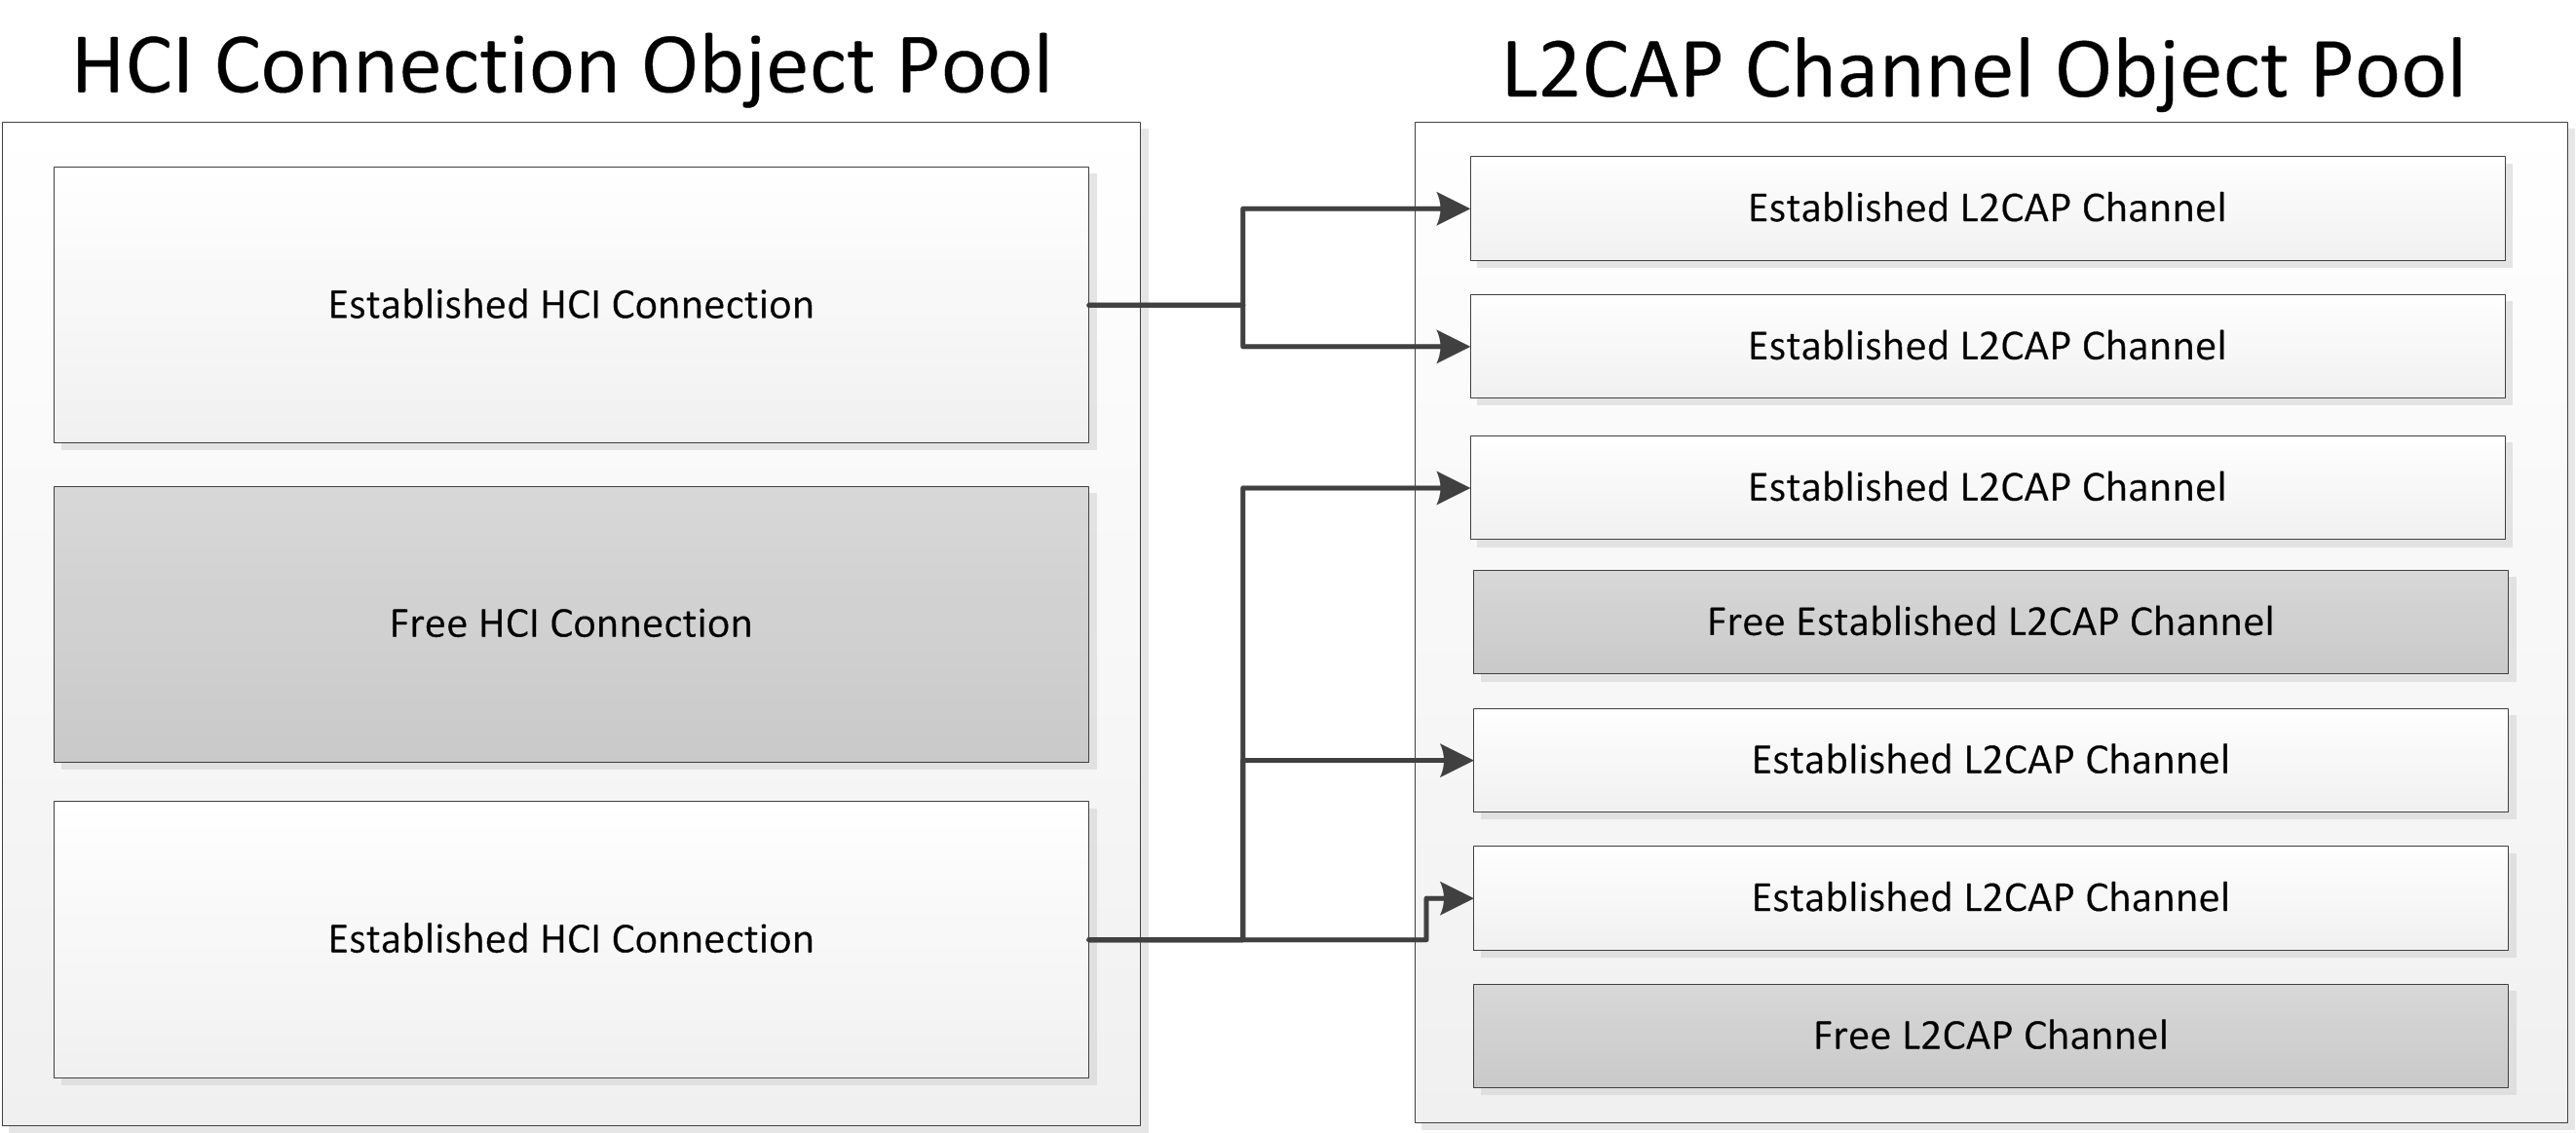
\includegraphics[width=140mm]{StackObjectPools.png}
	\rule{35em}{0.5pt}
	\caption[Diagram of the Bluetooth stack instance object pools]{Diagram showing the HCI Connection and L2CAP object pools within a single Bluetooth stack instance.}
	\label{fig:stackobjectpools}
\end{figure}

To positively link one used L2CAP channel instance to its parent HCI connection object, the HCI connection's \lstinline{handle} property is stored in the L2CAP channel object as a primary key. This handle value, allocated uniquely by the external Bluetooth HCI controller silicon when a new HCI connection is made, is then used to locate the HCI connection object within a stack instance from an established channel instance. While a pointer to the parent HCI object would offer a faster method of locating the associated HCI connection, this would tightly couple the HCI layer with the L2CAP layer as the former would need to alter the latter's objects if and when HCI connections are terminated.

As the stack does not use heap-based dynamic memory allocation, this approach ensures that the stack contains similar levels of flexibility to a dynamically allocated object approach, with only a minimal overhead. The maximum size of each object pool is set via the Bluetooth Stack's \lstinline{BT_MAX_DEVICE_CONNECTIONS} and \lstinline{BT_MAX_LOGICAL_CHANNELS} configuration defines.

\FloatBarrier
\subsection{Minimal Memory Usage}

While large embedded systems may run the completed Bluetooth stack, the design decisions made during its development were primarily aimed at ensuring the best performance and smallest footprint in severely resource-constrained microcontrollers. This resulted in the stack being optimised for small systems; only the minimal attributes required to establish and maintain connections are stored by the stack. One example of these optimizations is in the event system (described in detail later in this chapter) implementation: rather than implementing a callback registration system for each event, named callbacks are used instead. Various portions of the Bluetooth stack expect the user application to provide callback and event functions using names and prototypes defined in the stack header files.

This named callback function system reduces the memory footprint of the stack, as the callback addresses do not need to be stored in RAM at runtime, and the compiler does not need to inflate the binary with additional functions to manage the callback function registrations.

\section{Software Layer Implementation}

In this section, the design and implementation of each individual software layer that comprises the complete Bluetooth stack is described in detail.

\FloatBarrier
\subsection{Physical Transport}

While not part of the completed stack proper, a functional USB transport layer was completed for the project as an sample implementation in the user application, and hooked into the stack via the provided APIs. The Bluetooth USB transport \cite{bt2p1specs_usbtransport} requires the use of four logical USB communication channels (``pipes'' in USB terminology) to the USB Bluetooth adapter; the mandatory control pipe for HCI commands, a pair of \textit{Bulk} type pipes for data packets to and from the controller, and an \textit{Interrupt} pipe for HCI event notifications.

\begin{figure}[tbph]
	\vspace{1em}
	\centering
		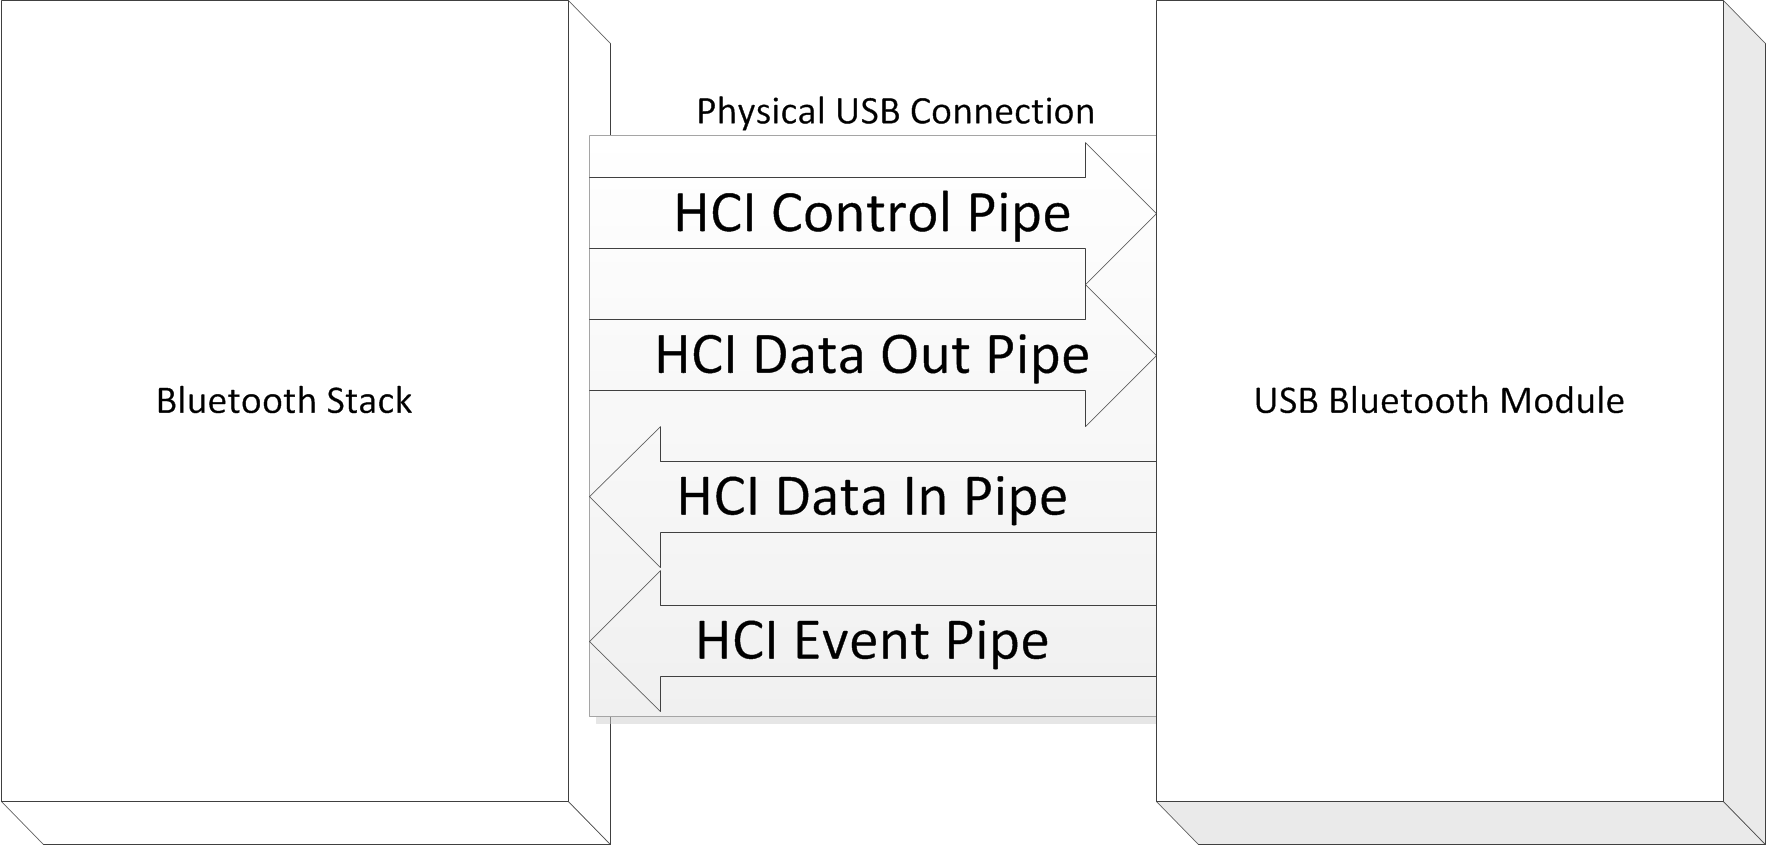
\includegraphics[width=100mm]{BluetoothUSBTransport.png}
	\rule{35em}{0.5pt}
	\caption[Diagram of the logical pipes within the Bluetooth USB transport.]{Diagram showing the logical USB pipes within the Bluetooth USB physical transport.}
	\label{fig:btusbtransport}
\end{figure}

Data and event packets received from the USB Bluetooth adapter's logical pipes are written into the packet buffer indicated in the stack instance configuration, and dispatched to the stack via the \lstinline{Bluetooth_ProcessPacket()} function. There they are processed internally via the Bluetooth stack, moving up the HCI, L2CAP and user-provided service layers as appropriate. The matching \lstinline{CALLBACK_Bluetooth_SendPacket()} callback function from the stack implements the data and HCI control packet transmission code back to the adapter, sourcing the generated packets from the same packet buffer location.

\FloatBarrier
\subsection{HCI Layer}

Sitting at the lowest level of the core stack, the HCI layer performs the main role of managing connections between Bluetooth devices, as well as processing events from the Bluetooth controller, and data encapsulation/decapsulation for transport over the Bluetooth link. To perform these tasks, the HCI layer is invoked each time a data packet is received or ready to be sent, an event is received from the controller, or during idle periods of the user application for general connection management.

The current HCI layer state is implemented as a state machine, which is automatically advanced through the appropriate states on stack initialization to configure the attached Bluetooth device, according to the configuration parameters set in the stack instance configuration structure. These states, shown in Listing \ref{lst:hcistates}, correspond to the asynchronous initialization steps performed by the stack when the HCI layer is reset.

\lstinputlisting[float=tbph,caption={State machine states for the HCI management layer.},label={lst:hcistates}]{./Figures/HCIStates.c}

The HCI baseband controller management in the HCI layer is split into two distinct parts; an event processing routine to process commands and manage transitions between HCI states, and the state machine processing routine to execute commands based on the current HCI state. As commands must only be sent once on the transition between HCI state machine states, a flag \lstinline{StateTransition} in the HCI state structure of each Bluetooth stack instance indicates if a state transition has occurred within the event processing function, so that the state machine processor can issue the appropriate responses on transition edges only.

State timeouts within each of the HCI states is managed via a \lstinline{TicksElapsed} counter in the HCI state structure of each Bluetooth stack instance. This counter, incremented each time the HCI layer is notified by the user application of a tick period elapsing, forces a resend of the current HCI state's command by forcing the state transition flag \lstinline{StateTransition} high when the timeout period has expired. This system ensures that HCI commands dropped during the initialisation of the module are properly re-issued.

If a connection is requested by a remote device, the HCI layer will issue a \\ \lstinline{CALLBACK_Bluetooth_ConnectionRequest()} callback into the user application, if space is available within the HCI connection object pool. If no space is available (i.e. all HCI channel objects are currently allocated for established connections) the connection request is silently discarded with the Bluetooth error code \lstinline{HCI_ERROR_LIMITED_RESOURCES}. If the user application accepts the connection request, the stack will issue an acceptance response to the remote device. If rejected, a suitable rejection notification is issued by the stack's HCI layer.

Authentication is currently implemented in a slave connection role only, as a PIN based authentication. All sent connection requests and acceptance packets indicate that the device requires a slave role in the connection establishment, indicating that the remote device is responsible for requesting the authentication PIN code from the user, which the local stack then authenticates against the PIN code configured in each stack instance.

Inside the HCI layer, received data packets are stripped of their HCI layer headers and passed upwards to the L2CAP layer for further processing. Packets sent from the L2CAP layer to the HCI layer undergo the opposite process; a HCI layer packet header is prefixed onto the packet contents and passed to the user application for transmission to the Bluetooth controller.

As an implementation-specific detail, HCI connection destruction events (when an established HCI connection is disconnected) are notified to the L2CAP layer via the internal function \lstinline{Bluetooth_L2CAP_NotifyHCIDisconnection()}. This ensures that all associated L2CAP channels are correctly destructed once their host HCI connection is destroyed, to prevent synchronisation issues and to ensure that the L2CAP object pool is freed of any dead channel objects as soon as possible to prevent unnecessary pool exhaustion.

\FloatBarrier
\subsection{L2CAP Layer}

The L2CAP layer, responsible for managing logical channels between devices for an established connection, was implemented in an unusual manner; due to uncertainties of the user application packet buffering scheme, the stack is not able to guarantee that packets to be sent are buffered correctly. As the L2CAP layer is used to establish communication channels between devices, it is essential that any issued channel configuration commands are delivered correctly to the remote device; delays in the channel negotiation process may cause communications to and from a remote device to fail. As a result, the L2CAP layer implemented a special event buffering scheme to ensure the reliable issuing of responses to remote devices even if a packet fails to send due to the controller's internal buffers becoming full.

As L2CAP signalling packets (identifiable via their destination channel ID of \texttt{0x0001}, the defined ID for \lstinline{BT_CHANNEL_SIGNALING} packets) are received by the L2CAP layer, the request is processed and an event object created in the L2CAP Event Queue. This queue, a fixed length queue of a size configured by the stack's \lstinline{BT_MAX_QUEUED_L2CAP_EVENTS} configuration parameter, stores the events in a First-In, First-Out ordered manner within each stack instance. The implementation of this queue is a simple flat array of event structure elements, where inserted items are appended to the end of the last allocated object in the array (see Figure \ref{fig:l2capeventinsertion}). A separate \lstinline{PendingEvents} property in the L2CAP state structure to track the number of queued events.

\begin{figure}[tbph]
	\vspace{1em}
	\centering
		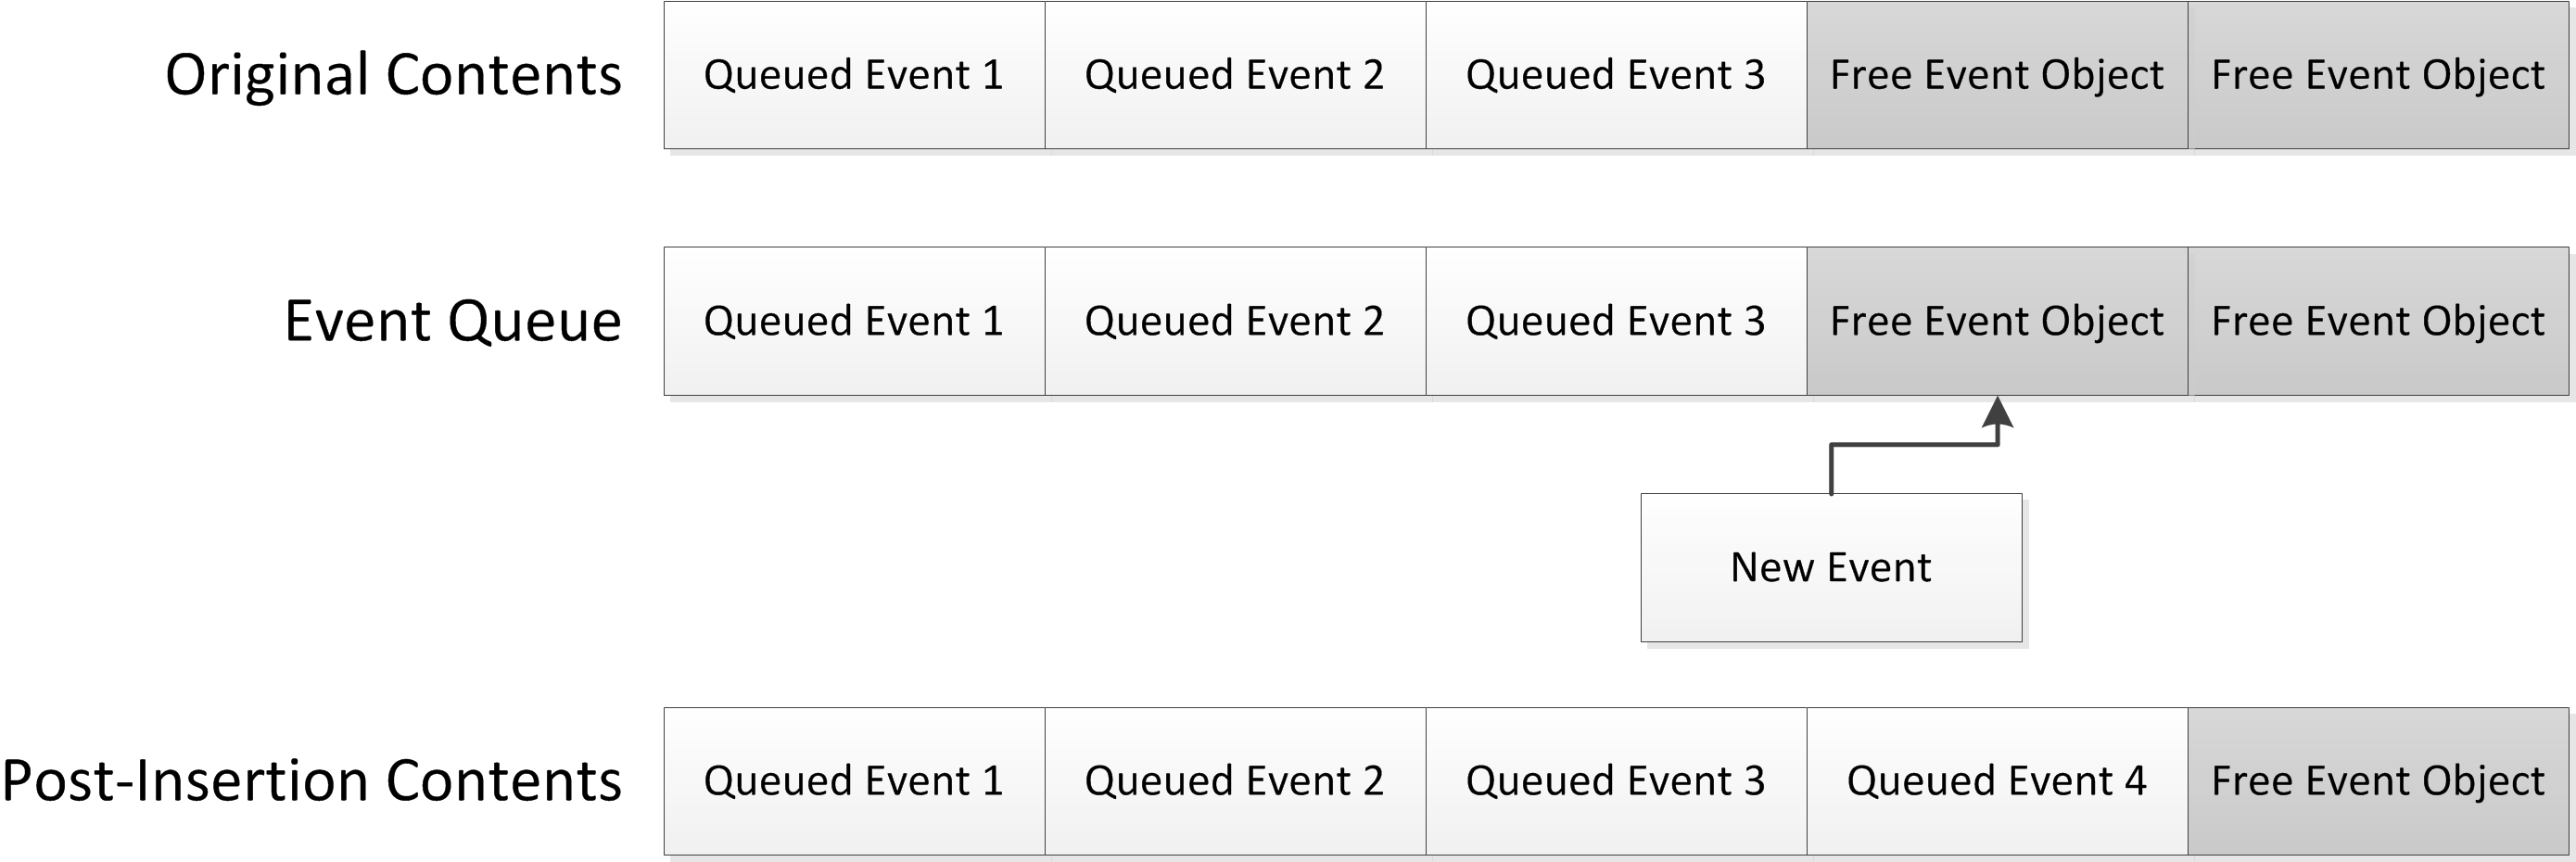
\includegraphics[width=140mm]{L2CAPEventInsertion.png}
	\rule{35em}{0.5pt}
	\caption[L2CAP Event Object Queue Insertion]{Diagram showing the insertion of a new L2CAP event into the tail of the queue.}
	\label{fig:l2capeventinsertion}
\end{figure}

Event queue removal is performed by the moving of all queue items above the head of the list leftwards in the array, to shuffle all entries one place towards the head of the queue (see Figure \ref{fig:l2capeventremoval}). L2CAP event objects are only dequeued once the transport layer confirms the transmission of the signalling packet request to the remote device. In this manner, L2CAP events maintain a reliable transport regardless of the physical transport's abilitiy to buffer excess packets.

\begin{figure}[tbph]
	\vspace{1em}
	\centering
		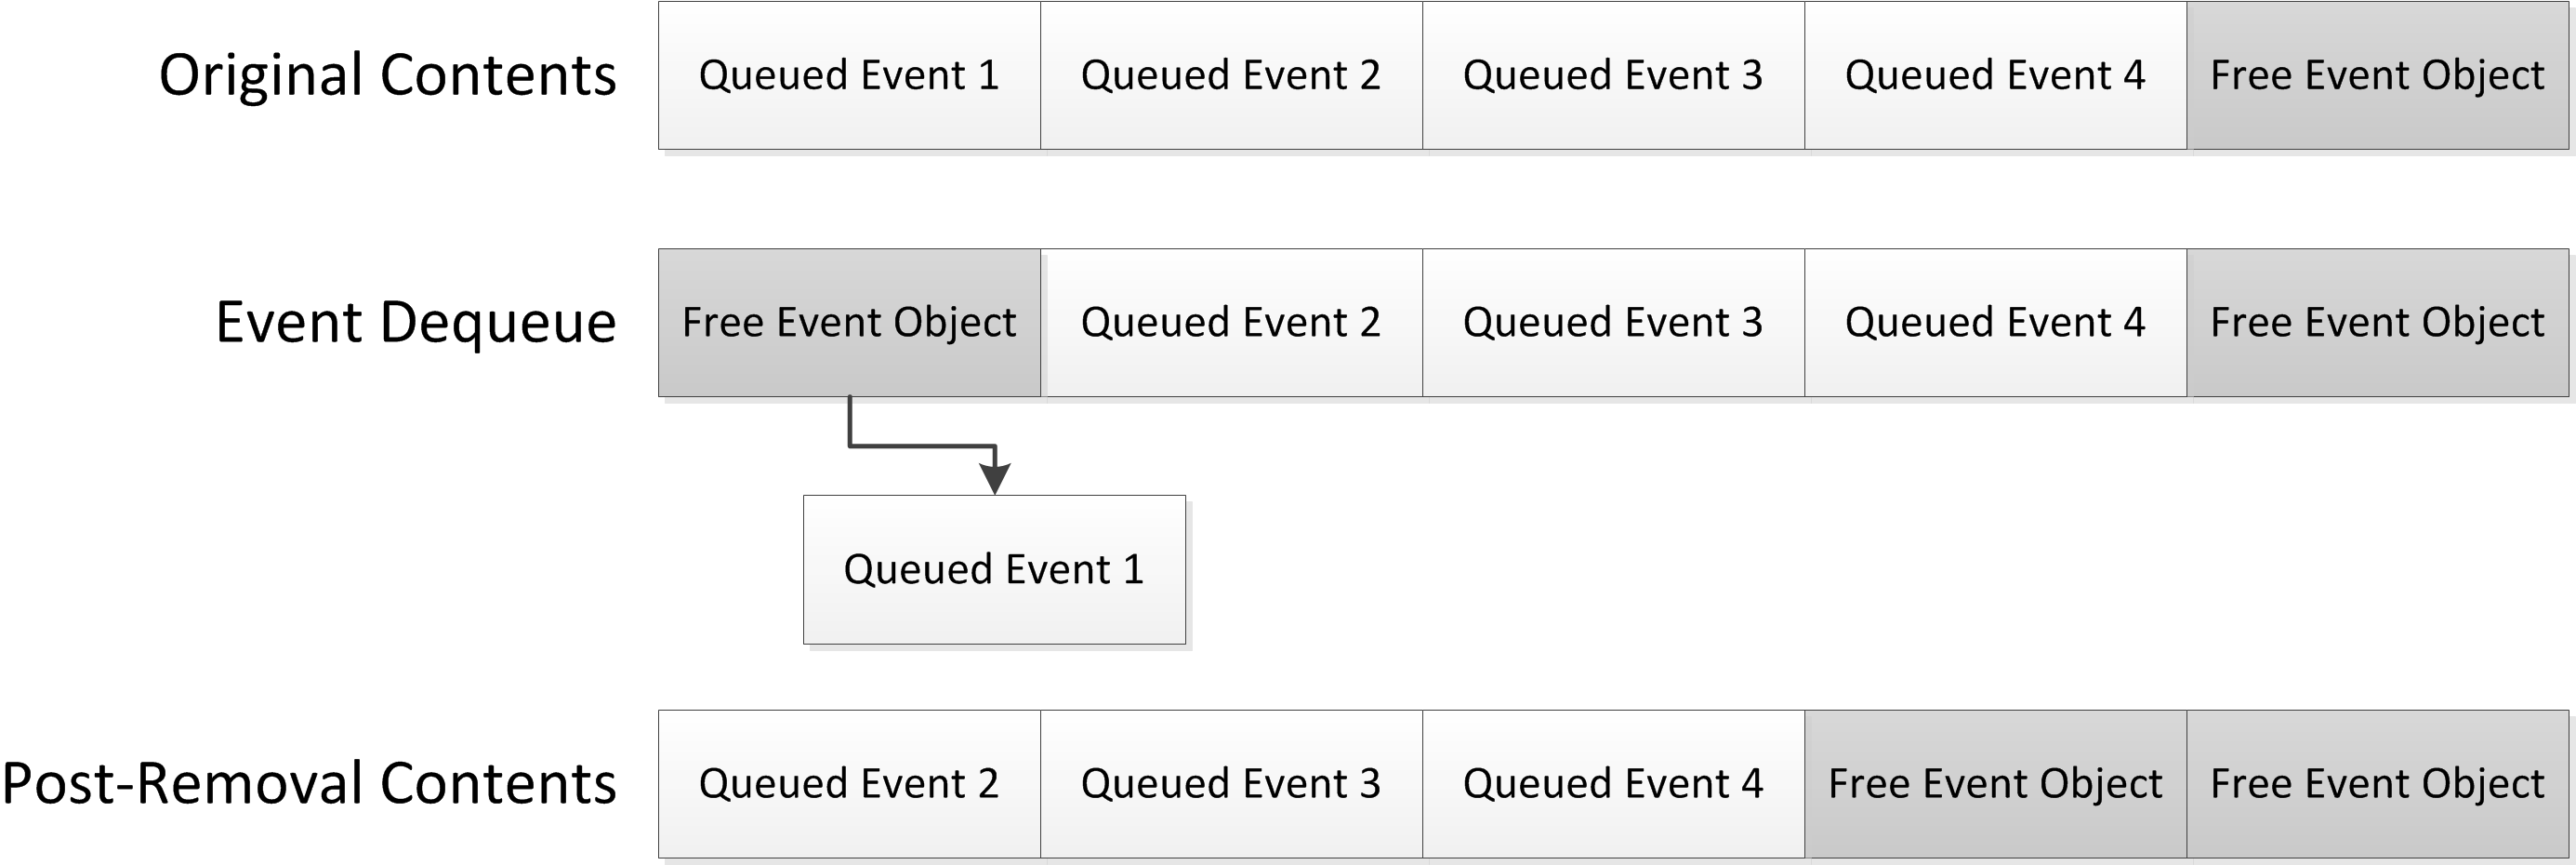
\includegraphics[width=140mm]{L2CAPEventRemoval.png}
	\rule{35em}{0.5pt}
	\caption[L2CAP Event Object Queue Removal]{Diagram showing the removal of the L2CAP event queue head item.}
	\label{fig:l2capeventremoval}
\end{figure}

If too many L2CAP events are attempted to be added to the queue, the new event allocation request will fail. This scheme will preserve existing events within the queue at the expense of dropping newer events until space becomes available. Despite this limitation, with an adequate queue size (of approximately 10 items for most applications) the queue limit should never be exceeded under normal circumstances.

\FloatBarrier
\subsection{Bluetooth Services}

The Bluetooth services designed as part of the project were implemented separately to the stack core; they are designed to hook into the stack APIs if desired by the user application, however they are entirely separate entities which are not required to be built with the stack core if not needed.

Bluetooth services can implement two possible roles; a \textit{client} role, or a \textit{server} role. It is possible for services to implement both roles, however this is not a requirement of the Bluetooth specification. Server role services (such as a Virtual Serial Port service server) provide a function to remote Bluetooth devices on demand, while client role services control remote service server instances (such as a termination application connecting to a remote Virtual Serial Port service server.)

Each of the services designed for the stack use a common set of interface APIs; functions are provided to the user application to notify the service of channel open/close events, data packet reception, and other such common events. In addition, each service may or may not expose a set of service-specific functions and callbacks, which can be used to interact with the service's functionality from the user application.

\FloatBarrier
\subsubsection{SDP Service}

For service discovery to take place between devices, each device must implement the Service Discovery Protocol service \cite{bt2p1specs_sdp}. The SDP service exposes the capabilities and characteristics of other services within the device, allowing remote systems to query the server to determine what services a device implements, and their associated properties. Other services may register themselves with the SDP service within a device, so that remote Bluetooth devices may detect the existence of the second service and make use of it if desired.

On large scale systems, SDP records are generally registered independently, and appropriate SDP records are built dynamically from the properties given to the SDP service by other services within a device. This approach allows for attributes to be dynamically added, removed and updated as required, however requires a variable amount of memory to store the generated SDP records. 

By contrast, the project's Bluetooth stack uses a novel static record initialization approach for SDP service attributes; services are required to contain pre-built SDP attribute records, which are then registered wholesale with the SDP server. While this requires complex SDP attribute tables to be built inside each service manually, this eliminates the need for costly run-time dynamic service record management and dynamic memory allocation.

An example of such a static SDP attribute record is shown in Listing \ref{lst:sdpattribute}. Here, a single UUID attribute is encoded in the correct format structure for the SDP server.

\lstinputlisting[float=tbph,caption={Example of a statically initialized SDP attribute.},label={lst:sdpattribute}]{./Figures/SDPAttribute.c}

In addition to each individual SDP attribute structure, a single Service Attribute Table must be built for each service requiring SDP registration. Listing \ref{lst:sdpattributetable} shows an example of a service's complete attribute table. When queried, the SDP server will example the attributes contained in this table to determine what (if any) attributes need to be returned to the requesting remote Bluetooth device.

\lstinputlisting[float=tbph,caption={Example of a statically initialized SDP attribute table.},label={lst:sdpattributetable}]{./Figures/SDPAttributeTable.c}

Finally for each service, a SDP entry node must be created. This master node is used to register the entire service and associated SDP attribute table with the SDP server. Listing \ref{lst:sdpentrynode} contains a sample SDP node.

\lstinputlisting[float=tbph,caption={Example of a statically initialized SDP service entry node.},label={lst:sdpentrynode}]{./Figures/SDPEntryNode.c}

The SDP server maintains a linked list of registered services internally, using the externally created SDP node entry instances. As services are registered and removed, these nodes are inserted and removed from the master SDP service list. When the SDP server is queried by a remote device, the server will transverse the list, looking for matching attributes to the request to return back to the initiating device.

\FloatBarrier
\subsubsection{RFCOMM Service}

For virtual serial port functionality, the RFCOMM service was implemented as a server role; remote devices can then request logical channels to be opened in the service, so that data can be exchanged. The RFCOMM service requires the creation of a logical channel multiplexer; this allows a single physical L2CAP channel to multiplex a collection of one or more RFCOMM data channels simultaneously. In the implementation of this service, the multiplexer was created using a static array of \lstinline{RFCOMM_Channel_t} structure instances, each of which represented a virtual channel on the multiplexer.

As the RFCOMM service is not tied directly into the core Bluetooth stack, the channel object array is not associated with a specific Bluetooth stack, rather, the channel object pool is shared amongst all Bluetooth stack instances in the system (see Figure \ref{fig:rfcommchannelpool}). The first time the service is initialised, the entire channel object pool is reset; in subsequent initializations, only channel objects currently associated to the stack instance being reset will be deallocated. This allows the RFCOMM service resources to be shared with all Bluetooth instances, without having to have multiple per-instance channel pools. The maximum number of simultaneously open RFCOMM channels is set via the \lstinline{RFCOMM_MAX_OPEN_CHANNELS} configuration parameter.

\begin{figure}[tbph]
	\vspace{1em}
	\centering
		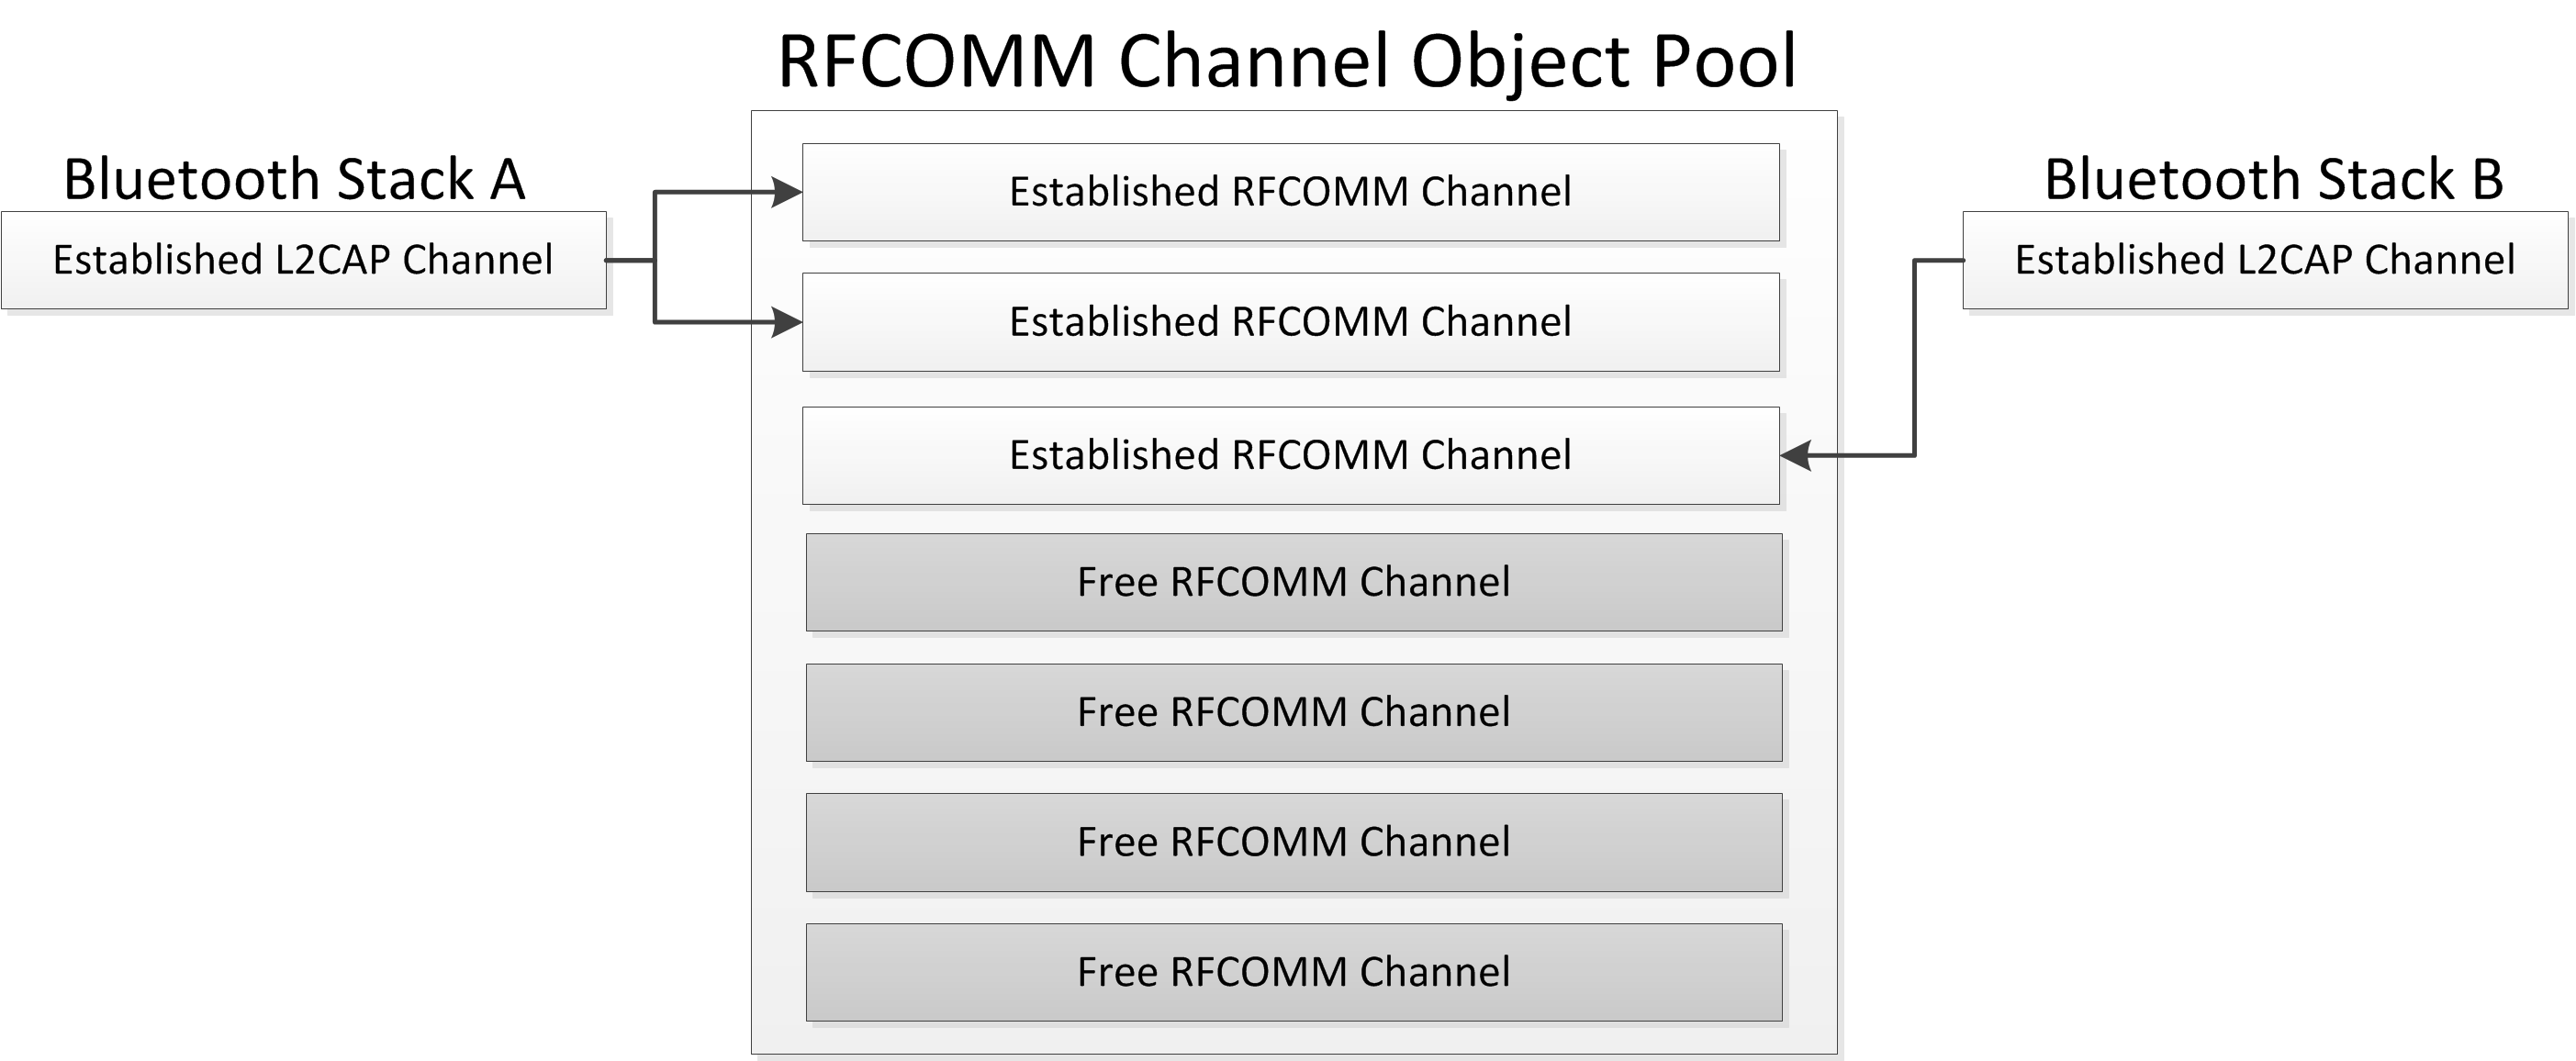
\includegraphics[width=140mm]{RFCOMMChannels.png}
	\rule{35em}{0.5pt}
	\caption[Diagram of the shared RFCOMM Channel pool.]{Diagram showing the RFCOMM channel object pool, shared amongst two Bluetooth stack instances.}
	\label{fig:rfcommchannelpool}
\end{figure}

While newer versions of the RFCOMM service specification (i.e. versions 1.1 onwards) add a mandatory ``credit based'' flow control scheme to control the flow of data in and out of each logical channel, versions 1.0B and earlier do not contain these additions. As most RFCOMM clients are compatible with either version (due to the prevalence of devices based on the older specification) the implemented service was based on the earlier protocol version \cite{rfcommspecs} for simplicity.

\FloatBarrier
\subsubsection{HID Service}

Due to time limitations of the project, the HID service implementation was extremely minimal; only a basic implementation of the HID 1.0 profile \cite{bthidspecs} was designed and coded, so that received packets could be decoded and used to control the robot. As a client role version of the SDP server was not attempted, the HID service was unable to query the remote HID device's service tables for the HID descriptor, used to determine how to decode received HID data packets. This unfortunately resulted in the final robot firmware needing to hard-code the packet interpretation for each device type based on the length of the received data packet.

\section{Integration into User Applications}

In order to implement the Bluetooth stack into a user application, the entire base stack (excluding the services) must be added to the project for compilation. The user configuration and interface to the stack is made via the header file \texttt{BluetoothCommon.h}. User applications attempting to use the stack must be compiled using the C99 language specification, and a GCC compiler derivative.

\FloatBarrier
\subsection{Management Functions}

The following functions must be executed by the user application to operate the stack correctly.

\vspace{1em}
\begin{lstlisting}
	void Bluetooth_Init(BT_StackConfig_t* const StackState);
\end{lstlisting}

The stack initialization function must be called once on system startup, to initialize a given instance of the stack ready for use.

\vspace{1em}
\begin{lstlisting}
	bool Bluetooth_ManageConnections(BT_StackConfig_t* const StackState);
\end{lstlisting}

This function must be executed periodically to manage existing connections and reply to any pending L2CAP or HCI events. The exact frequency this function must be called at is not a concrete value, rather, it should be called as fast as the user application will allow. Failure to call this function fast enough will introduce latency when establishing and maintaining new connections and logical channels or, in extreme cases, will cause connection and channel negotiations to fail.
	
\vspace{1em}
\begin{lstlisting}
	void Bluetooth_ProcessPacket(BT_StackConfig_t* const StackState,
	                             const uint8_t Type);
\end{lstlisting}

When a new packet is received from the Bluetooth controller, this function must be invoked. Note that the received packet data should be stored into the packet buffer set in the Bluetooth stack instance's configuration structure prior to invoking the packet processing routine.

\vspace{1em}
\begin{lstlisting}
	void Bluetooth_TickElapsed(BT_StackConfig_t* const StackState);
\end{lstlisting}

To manage timeouts, the stack must be updated regularly of the passage of time using this function. Each time the configured \lstinline{BT_TICK_MS} tick period elapses, this function should be invoked to determine if any timeout conditions must be generated internally.

\FloatBarrier
\subsection{Events and Callbacks}

In response to conditions set within the stack internals, one or more event or callback functions may be invoked. These functions, implemented by the user application, allow the system to respond to events in a synchronous manner as they occur within the stack, and/or indicate to the stack the appropriate action to take when a decision is required. The user-implemented functions are split into two categories:

\begin{enumerate}
	\item \textbf{Event Functions}, which allow the user application to respond to events. This class of function has no return value, and the user application may choose to not provide a functional implementation for one or more events, if the event condition is of no interest to the user application.
	\item \textbf{Callback Functions}, invoked when the stack reaches a condition where a decision must be made by the user application---such as whether to accept or reject a particular incoming connection or channel request---before stack operations can continue. These functions require a decision to be give as the function's return value, which is then used by the stack internally.
\end{enumerate}

Event and callback invocations are generated by the stack layers as required. Figure \ref{fig:messageresponsecallback} shows the general message, callback and response sequence path a typical software stack will follow throughout its normal processing activities.

\begin{figure}[tbph]
	\vspace{1em}
	\centering
		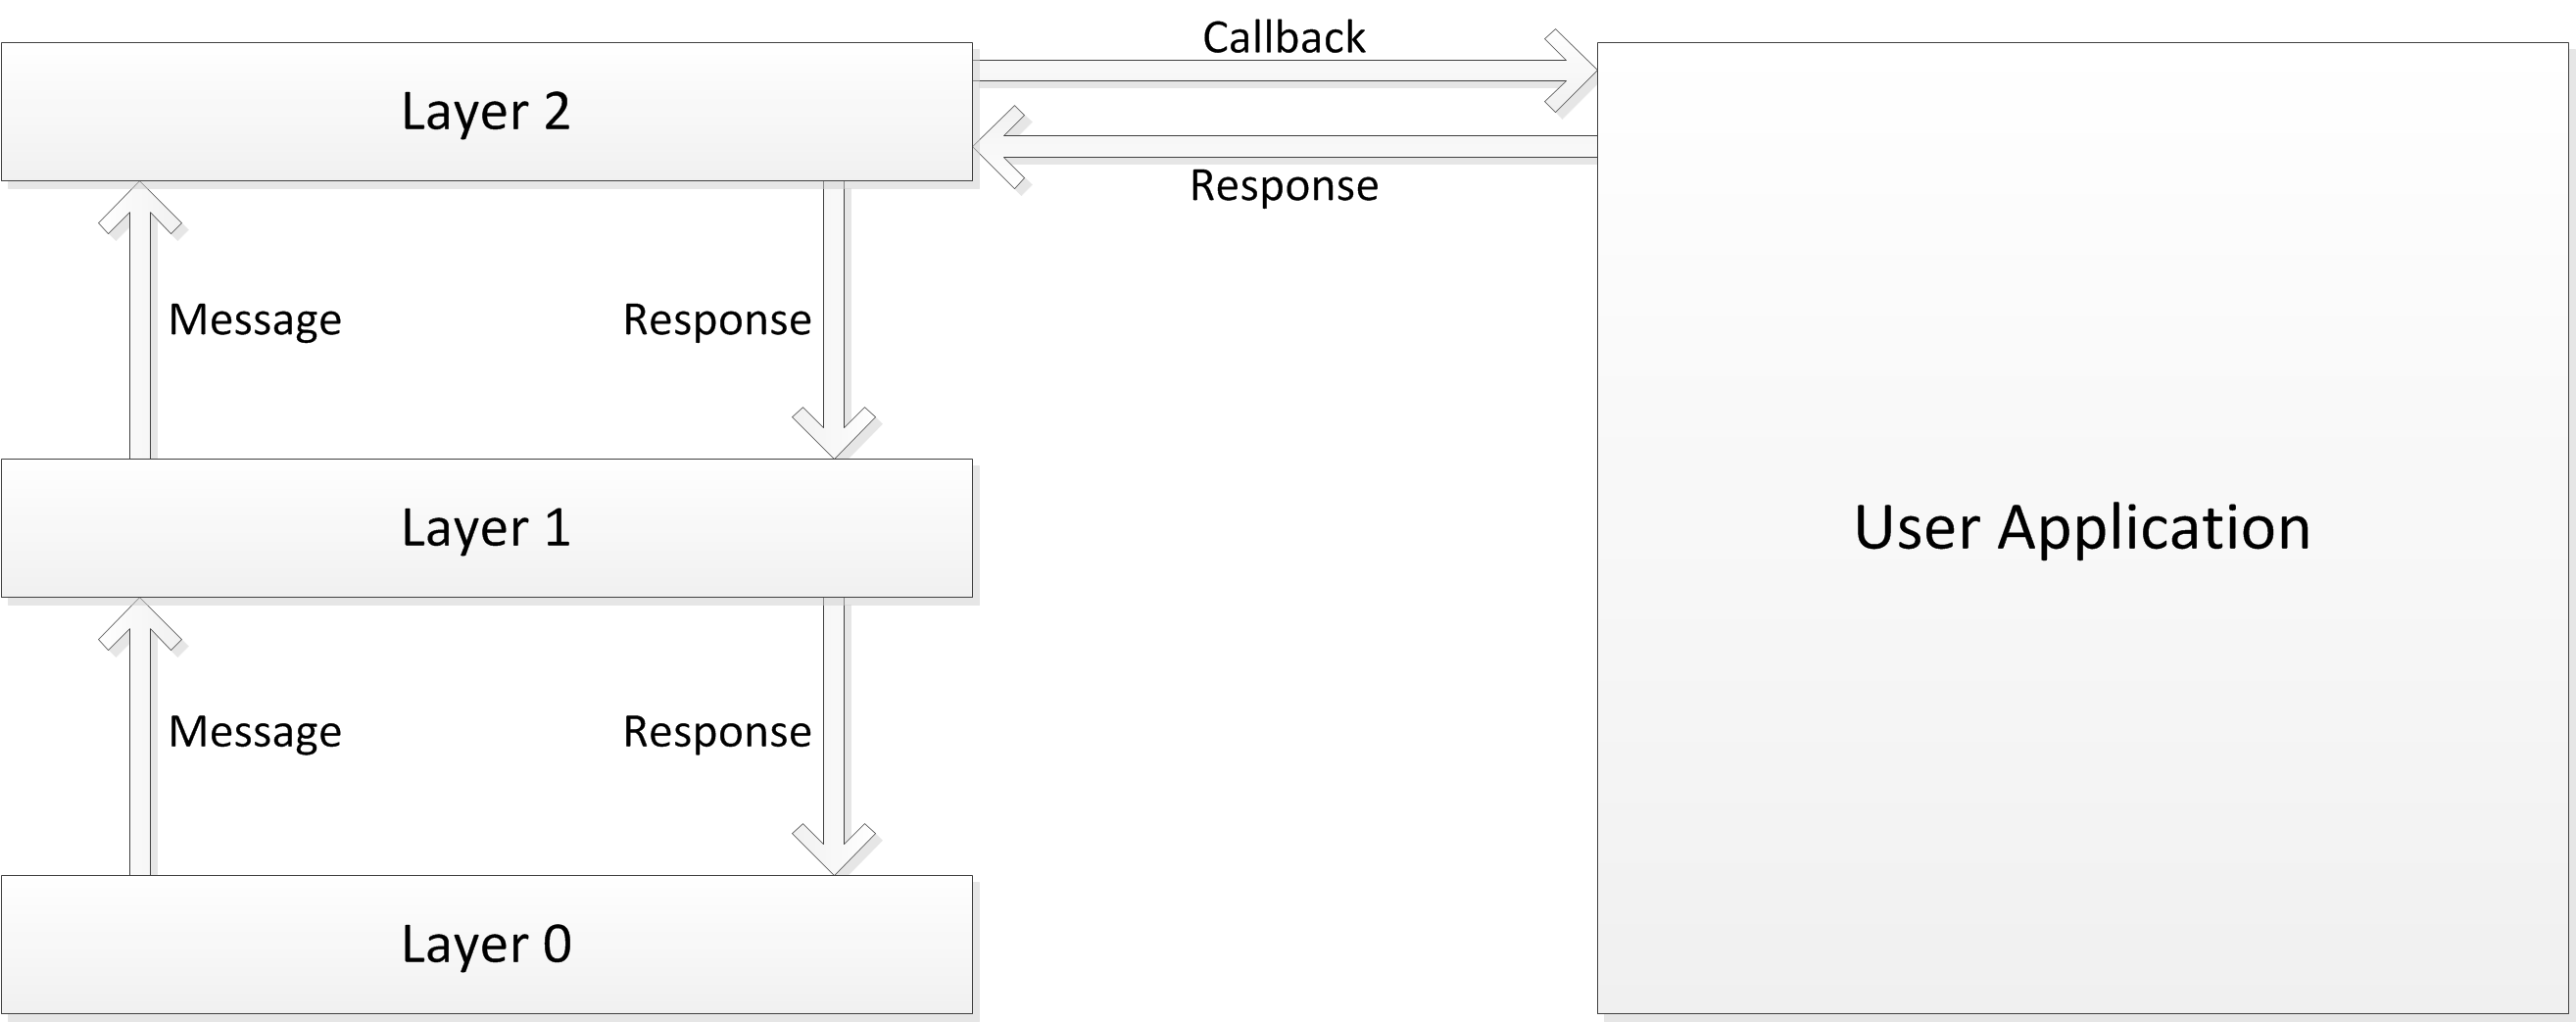
\includegraphics[width=140mm]{MessageResponseCallback.png}
	\rule{35em}{0.5pt}
	\caption[Diagram of the Message, Response and Callback sequence]{Diagram showing the Message, Response and Callback sequence of a typical software stack when passing a message and response through several intermediate layers.}
	\label{fig:messageresponsecallback}
\end{figure}

In the project's Bluetooth stack, the names of the event and callback functions are fixed, and cannot be changed. User applications are required to implement all callback and event functions (identified via their \lstinline{CALLBACK_} and \lstinline{EVENT_} prefixes) using the exact prototypes given in the module headers. This design was preferred over a traditional registration system to reduce the stack's binary size and RAM footprint.

A minimal set of callback and event functions (excluding the physical packet transport callback) required to link in the SDP and RFCOMM services to the core Bluetooth stack are shown in Listing \ref{lst:minbteventcallbacks}.

\lstinputlisting[float=tbph,caption={Minimal set of event callbacks for SDP and RFCOMM service use.},label={lst:minbteventcallbacks}]{./Figures/MinimalBTEventCallbacks.c}
